\documentclass[12pt,]{krantz}
\usepackage{lmodern}
\usepackage{amssymb,amsmath}
\usepackage{ifxetex,ifluatex}
\usepackage{fixltx2e} % provides \textsubscript
\ifnum 0\ifxetex 1\fi\ifluatex 1\fi=0 % if pdftex
  \usepackage[T1]{fontenc}
  \usepackage[utf8]{inputenc}
\else % if luatex or xelatex
  \ifxetex
    \usepackage{mathspec}
  \else
    \usepackage{fontspec}
  \fi
  \defaultfontfeatures{Ligatures=TeX,Scale=MatchLowercase}
\fi
% use upquote if available, for straight quotes in verbatim environments
\IfFileExists{upquote.sty}{\usepackage{upquote}}{}
% use microtype if available
\IfFileExists{microtype.sty}{%
\usepackage{microtype}
\UseMicrotypeSet[protrusion]{basicmath} % disable protrusion for tt fonts
}{}
\usepackage[margin=1in]{geometry}
\usepackage{hyperref}
\PassOptionsToPackage{usenames,dvipsnames}{color} % color is loaded by hyperref
\hypersetup{unicode=true,
            pdftitle={R을 통한 비구획분석: 실습},
            pdfauthor={서울아산병원 임상약리학과 전공의 한성필},
            colorlinks=true,
            linkcolor=Maroon,
            citecolor=Blue,
            urlcolor=Blue,
            breaklinks=true}
\urlstyle{same}  % don't use monospace font for urls
\usepackage{color}
\usepackage{fancyvrb}
\newcommand{\VerbBar}{|}
\newcommand{\VERB}{\Verb[commandchars=\\\{\}]}
\DefineVerbatimEnvironment{Highlighting}{Verbatim}{commandchars=\\\{\}}
% Add ',fontsize=\small' for more characters per line
\usepackage{framed}
\definecolor{shadecolor}{RGB}{248,248,248}
\newenvironment{Shaded}{\begin{snugshade}}{\end{snugshade}}
\newcommand{\KeywordTok}[1]{\textcolor[rgb]{0.13,0.29,0.53}{\textbf{#1}}}
\newcommand{\DataTypeTok}[1]{\textcolor[rgb]{0.13,0.29,0.53}{#1}}
\newcommand{\DecValTok}[1]{\textcolor[rgb]{0.00,0.00,0.81}{#1}}
\newcommand{\BaseNTok}[1]{\textcolor[rgb]{0.00,0.00,0.81}{#1}}
\newcommand{\FloatTok}[1]{\textcolor[rgb]{0.00,0.00,0.81}{#1}}
\newcommand{\ConstantTok}[1]{\textcolor[rgb]{0.00,0.00,0.00}{#1}}
\newcommand{\CharTok}[1]{\textcolor[rgb]{0.31,0.60,0.02}{#1}}
\newcommand{\SpecialCharTok}[1]{\textcolor[rgb]{0.00,0.00,0.00}{#1}}
\newcommand{\StringTok}[1]{\textcolor[rgb]{0.31,0.60,0.02}{#1}}
\newcommand{\VerbatimStringTok}[1]{\textcolor[rgb]{0.31,0.60,0.02}{#1}}
\newcommand{\SpecialStringTok}[1]{\textcolor[rgb]{0.31,0.60,0.02}{#1}}
\newcommand{\ImportTok}[1]{#1}
\newcommand{\CommentTok}[1]{\textcolor[rgb]{0.56,0.35,0.01}{\textit{#1}}}
\newcommand{\DocumentationTok}[1]{\textcolor[rgb]{0.56,0.35,0.01}{\textbf{\textit{#1}}}}
\newcommand{\AnnotationTok}[1]{\textcolor[rgb]{0.56,0.35,0.01}{\textbf{\textit{#1}}}}
\newcommand{\CommentVarTok}[1]{\textcolor[rgb]{0.56,0.35,0.01}{\textbf{\textit{#1}}}}
\newcommand{\OtherTok}[1]{\textcolor[rgb]{0.56,0.35,0.01}{#1}}
\newcommand{\FunctionTok}[1]{\textcolor[rgb]{0.00,0.00,0.00}{#1}}
\newcommand{\VariableTok}[1]{\textcolor[rgb]{0.00,0.00,0.00}{#1}}
\newcommand{\ControlFlowTok}[1]{\textcolor[rgb]{0.13,0.29,0.53}{\textbf{#1}}}
\newcommand{\OperatorTok}[1]{\textcolor[rgb]{0.81,0.36,0.00}{\textbf{#1}}}
\newcommand{\BuiltInTok}[1]{#1}
\newcommand{\ExtensionTok}[1]{#1}
\newcommand{\PreprocessorTok}[1]{\textcolor[rgb]{0.56,0.35,0.01}{\textit{#1}}}
\newcommand{\AttributeTok}[1]{\textcolor[rgb]{0.77,0.63,0.00}{#1}}
\newcommand{\RegionMarkerTok}[1]{#1}
\newcommand{\InformationTok}[1]{\textcolor[rgb]{0.56,0.35,0.01}{\textbf{\textit{#1}}}}
\newcommand{\WarningTok}[1]{\textcolor[rgb]{0.56,0.35,0.01}{\textbf{\textit{#1}}}}
\newcommand{\AlertTok}[1]{\textcolor[rgb]{0.94,0.16,0.16}{#1}}
\newcommand{\ErrorTok}[1]{\textcolor[rgb]{0.64,0.00,0.00}{\textbf{#1}}}
\newcommand{\NormalTok}[1]{#1}
\usepackage{longtable,booktabs}
\usepackage{graphicx,grffile}
\makeatletter
\def\maxwidth{\ifdim\Gin@nat@width>\linewidth\linewidth\else\Gin@nat@width\fi}
\def\maxheight{\ifdim\Gin@nat@height>\textheight\textheight\else\Gin@nat@height\fi}
\makeatother
% Scale images if necessary, so that they will not overflow the page
% margins by default, and it is still possible to overwrite the defaults
% using explicit options in \includegraphics[width, height, ...]{}
\setkeys{Gin}{width=\maxwidth,height=\maxheight,keepaspectratio}
\IfFileExists{parskip.sty}{%
\usepackage{parskip}
}{% else
\setlength{\parindent}{0pt}
\setlength{\parskip}{6pt plus 2pt minus 1pt}
}
\setlength{\emergencystretch}{3em}  % prevent overfull lines
\providecommand{\tightlist}{%
  \setlength{\itemsep}{0pt}\setlength{\parskip}{0pt}}
\setcounter{secnumdepth}{5}
% Redefines (sub)paragraphs to behave more like sections
\ifx\paragraph\undefined\else
\let\oldparagraph\paragraph
\renewcommand{\paragraph}[1]{\oldparagraph{#1}\mbox{}}
\fi
\ifx\subparagraph\undefined\else
\let\oldsubparagraph\subparagraph
\renewcommand{\subparagraph}[1]{\oldsubparagraph{#1}\mbox{}}
\fi

%%% Use protect on footnotes to avoid problems with footnotes in titles
\let\rmarkdownfootnote\footnote%
\def\footnote{\protect\rmarkdownfootnote}

%%% Change title format to be more compact
\usepackage{titling}

% Create subtitle command for use in maketitle
\newcommand{\subtitle}[1]{
  \posttitle{
    \begin{center}\large#1\end{center}
    }
}

\setlength{\droptitle}{-2em}
  \title{R을 통한 비구획분석: 실습}
  \pretitle{\vspace{\droptitle}\centering\huge}
  \posttitle{\par}
  \author{서울아산병원 임상약리학과 전공의 한성필}
  \preauthor{\centering\large\emph}
  \postauthor{\par}
  \predate{\centering\large\emph}
  \postdate{\par}
  \date{2017-11-14}

\usepackage{kotex}

\begin{document}
\maketitle

{
\hypersetup{linkcolor=black}
\setcounter{tocdepth}{2}
\tableofcontents
}
\mainmatter

\hypertarget{intro}{%
\chapter{서론}\label{intro}}

약동학 분야에서 가장 간단하고도 객관적이며 널리 쓰이는 방법은 비구획분석
(Non-compartmental analysis, NCA)입니다. \emph{미국의 FDA (Food and Drug
Administration)를 비롯한 대부분의 규제기관에서는 NCA하는 소프트웨어를
규정하고 있지 않아}, 상용 소프트웨어를 사용하지 않고 약동학적 지표를
구하는 것을 허용하고 있습니다. 따라서 무료로 누구나 사용할 수 있는 R
패키지를 사용하여 비구획분석을 통한 약동학적 주요 지표를 구할 수
있습니다.

\begin{itemize}
\tightlist
\item
  NonCompart (Bae
  \protect\hyperlink{ref-R-NonCompart}{2017}\protect\hyperlink{ref-R-NonCompart}{b})
\item
  ncar (Bae
  \protect\hyperlink{ref-R-ncar}{2017}\protect\hyperlink{ref-R-ncar}{a})
\item
  pkr (Bae and Lee \protect\hyperlink{ref-R-pkr}{2017})
\end{itemize}

\section{설치}

우선 R을 설치합니다. R은 아래 링크\footnote{\url{https://cran.r-project.org/}}에서
다운로드 받을 수 있습니다.

R을 실행한 후, 콘솔 창에서 비구획분석을 위한 패키지를 설치하는 방법은
다음과 같습니다. 홑따옴표 등의 인용 부호에 주의하세요.

\begin{Shaded}
\begin{Highlighting}[]
\KeywordTok{install.packages}\NormalTok{(}\StringTok{'NonCompart'}\NormalTok{)}
\KeywordTok{install.packages}\NormalTok{(}\StringTok{'ncar'}\NormalTok{)}
\KeywordTok{install.packages}\NormalTok{(}\StringTok{'pkr'}\NormalTok{)}
\end{Highlighting}
\end{Shaded}

설치는 한번만 하면 되지만, 비구획분석을 위해서는 매 세션마다 패키지를
\emph{불러오기}해야 합니다.

\begin{Shaded}
\begin{Highlighting}[]
\KeywordTok{library}\NormalTok{(NonCompart)}
\KeywordTok{library}\NormalTok{(ncar)}
\KeywordTok{library}\NormalTok{(pkr)}
\end{Highlighting}
\end{Shaded}

아래 두 패키지는 비구획분석과는 관계없지만 자료 처리 혹은 그림 등을
그리는데 도움을 줍니다.

\begin{Shaded}
\begin{Highlighting}[]
\CommentTok{# install.packages(c('tidyverse', 'knitr')) # 설치 안되어 있으면 맨앞의 #을 지우고 설치.}
\KeywordTok{library}\NormalTok{(tidyverse) }\CommentTok{# For presentation only, dplyr, tidyr, ggplot2}
\KeywordTok{library}\NormalTok{(knitr) }\CommentTok{# For reports}
\end{Highlighting}
\end{Shaded}

도움이 필요할때는 맨 앞에 물음표를 붙여서 콘솔창에 입력하거나
\texttt{help()} 함수를 사용합니다.

\begin{Shaded}
\begin{Highlighting}[]
\NormalTok{?NonCompart}
\KeywordTok{help}\NormalTok{(tblNCA)}
\end{Highlighting}
\end{Shaded}

\hypertarget{r-}{%
\section{R에 대하여}\label{r-}}

R (R Core Team \protect\hyperlink{ref-R-base}{2017})은 통계 소프트웨어
입니다. 굉장히 유용한 소프트웨어이지만 이에 대해 여기서 자세히 설명하긴
힘듭니다. R에 대한 많은 책들을 bookdown.org\footnote{\url{https://bookdown.org}}에서
무료로 읽을 수 있습니다. Coursera\footnote{\url{https://coursera.com}}에서
무료 온라인 강의를 들을 수 있습니다.

\hypertarget{-}{%
\section{자료 탐색}\label{-}}

자료의 첫 10개 (Table \ref{tab:head}) 혹은 마지막 10개 관찰값만 보고
싶으면 다음을 입력합니다. 대상자 번호가 첫 열에 나와있고 시간 순서대로
혈장에서 측정한 테오필린의 농도가 나와있습니다.

\begin{Shaded}
\begin{Highlighting}[]
\KeywordTok{head}\NormalTok{(Theoph, }\DataTypeTok{n=}\DecValTok{10}\NormalTok{)}
\KeywordTok{tail}\NormalTok{(Theoph, }\DataTypeTok{n=}\DecValTok{10}\NormalTok{)}
\end{Highlighting}
\end{Shaded}

\begin{table}

\caption{\label{tab:head}Theoph 자료의 첫 10개 관찰값}
\centering
\begin{tabular}[t]{lrrrr}
\toprule
Subject & Wt & Dose & Time & conc\\
\midrule
1 & 79.6 & 4.02 & 0.00 & 0.74\\
1 & 79.6 & 4.02 & 0.25 & 2.84\\
1 & 79.6 & 4.02 & 0.57 & 6.57\\
1 & 79.6 & 4.02 & 1.12 & 10.50\\
1 & 79.6 & 4.02 & 2.02 & 9.66\\
\addlinespace
1 & 79.6 & 4.02 & 3.82 & 8.58\\
1 & 79.6 & 4.02 & 5.10 & 8.36\\
1 & 79.6 & 4.02 & 7.03 & 7.47\\
1 & 79.6 & 4.02 & 9.05 & 6.89\\
1 & 79.6 & 4.02 & 12.12 & 5.94\\
\bottomrule
\end{tabular}
\end{table}

그림을 그려서 대략적인 자료의 모습을 파악합니다. (Figure
\ref{fig:ggtheoph})

\begin{Shaded}
\begin{Highlighting}[]
\KeywordTok{ggplot}\NormalTok{(Theoph, }\KeywordTok{aes}\NormalTok{(Time, conc, }\DataTypeTok{group =}\NormalTok{ Subject, }\DataTypeTok{color =}\NormalTok{ Subject)) }\OperatorTok{+}
\StringTok{  }\KeywordTok{geom_point}\NormalTok{(}\DataTypeTok{size =} \DecValTok{4}\NormalTok{) }\OperatorTok{+}\StringTok{ }
\StringTok{  }\KeywordTok{geom_line}\NormalTok{(}\DataTypeTok{size =} \DecValTok{1}\NormalTok{) }\OperatorTok{+}
\StringTok{  }\KeywordTok{theme_bw}\NormalTok{() }\OperatorTok{+}
\StringTok{  }\KeywordTok{labs}\NormalTok{(}\DataTypeTok{title =} \StringTok{'Oral Administration of Theoph (320 mg)'}\NormalTok{,}
       \DataTypeTok{x =} \StringTok{'Time (hour)'}\NormalTok{, }\DataTypeTok{y =} \StringTok{'Concentration (ng/mL)'}\NormalTok{)}
\end{Highlighting}
\end{Shaded}

\begin{figure}
\centering
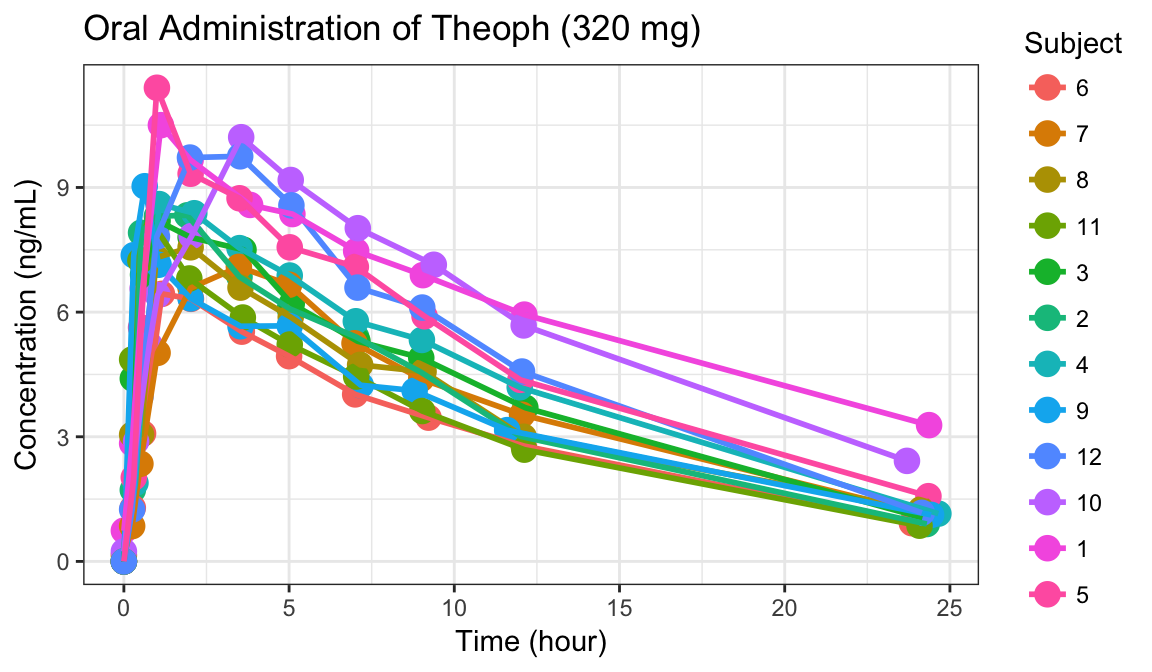
\includegraphics{handout_files/figure-latex/ggtheoph-1.pdf}
\caption{\label{fig:ggtheoph}Concentration-time curves of oral
administration of Theoph (N = 12)}
\end{figure}

\hypertarget{-}{%
\section{파라메터의 의미}\label{-}}

비구획분석 시 여러 파라메터가 나오며 약어로 표현하는 경우가 많습니다.
또한 소프트웨어마다 약어가 상이하기 때문에 자주 그 의미를 찾아볼 필요가
있습니다. 콘솔창에 다음을 입력합니다.

\begin{Shaded}
\begin{Highlighting}[]
\NormalTok{?ncar}\OperatorTok{::}\KeywordTok{txtNCA}\NormalTok{()}
\NormalTok{ncar}\OperatorTok{::}\NormalTok{RptCfg}
\end{Highlighting}
\end{Shaded}

ncar::RptCfg의 일부를 첨부합니다. (Table \ref{tab:rptcfg})
\texttt{PPTESTCD}는 NonCompart 패키지에서 출력하는 파라메터 이름이며,
CDISC SDTM PPTESTCD (Parameter Short Name)\footnote{다음과 같이 CDISC
  note에 표시되어 있습니다. `Short name of the pharmacokinetic
  parameter. It can be used as a column name when converting a dataset
  from a vertical to a horizontal format. The value in PPTESTCD cannot
  be longer than 8 characters, nor can it start with a number (e.g.,
  ``1TEST''). PPTESTCD cannot contain characters other than letters,
  numbers, or underscores. Examples: ``AUCALL'', ``TMAX'', ``CMAX''.'
  \url{https://wiki.cdisc.org/pages/viewpage.action?pageId=42309513}}와
같은 값입니다. \texttt{WNL} 열은 Certara Phoenix WinNonLin에서 구한
파라메터 이름입니다.

\begin{longtable}[t]{lll}
\caption{\label{tab:rptcfg}Description of NonCompart parameters}\\
\toprule
PPTESTCD & SYNONYM & WNL\\
\midrule
b0 & Intercept & b0\\
TLAG & Time Until First Nonzero Conc & Tlag\\
MRTEVLST & MRT Extravasc to Last Nonzero Conc & MRTlast\\
MRTEVIFO & MRT Extravasc Infinity Obs & MRTINF\_obs\\
MRTEVIFP & MRT Extravasc Infinity Pred & MRTINF\_pred\\
\addlinespace
VZFO & Vz Obs by F & Vz\_F\_obs\\
VZFP & Vz Pred by F & Vz\_F\_pred\\
CLFO & Total CL Obs by F & Cl\_F\_obs\\
CLFP & Total CL Pred by F & Cl\_F\_pred\\
C0 & Initial Conc & C0\\
\addlinespace
AUCPBEO & AUC \%Back Extrapolation Obs & AUC\_.Back\_Ext\_obs\\
AUCPBEP & AUC \%Back Extrapolation Pred & AUC\_.Back\_Ext\_pred\\
CMAX & Max Conc & Cmax\\
CMAXD & Max Conc Norm by Dose & Cmax\_D\\
TMAX & Time of CMAX & Tmax\\
\addlinespace
CLST & Last Nonzero Conc & Clast\\
TLST & Time of Last Nonzero Conc & Tlast\\
CLSTP & Last Nonzero Conc Pred & Clast\_pred\\
LAMZHL & Half-Life Lambda z & HL\_Lambda\_z\\
LAMZ & Lambda z & Lambda\_z\\
\addlinespace
LAMZLL & Lambda z Lower Limit & Lambda\_z\_lower\\
LAMZUL & Lambda z Upper Limit & Lambda\_z\_upper\\
LAMZNPT & Number of Points for Lambda z & No\_points\_lambda\_z\\
CORRXY & Correlation Between TimeX and Log ConcY & Corr\_XY\\
R2 & R Squared & Rsq\\
\addlinespace
R2ADJ & R Squared Adjusted & Rsq\_adjusted\\
AUCLST & AUC to Last Nonzero Conc & AUClast\\
AUCALL & AUC All & AUCall\\
AUCIFO & AUC Infinity Obs & AUCINF\_obs\\
AUCIFOD & AUC Infinity Obs Norm by Dose & AUCINF\_D\_obs\\
\addlinespace
AUCPEO & AUC \%Extrapolation Obs & AUC\_.Extrap\_obs\\
AUCIFP & AUC Infinity Pred & AUCINF\_pred\\
AUCIFPD & AUC Infinity Pred Norm by Dose & AUCINF\_D\_pred\\
AUCPEP & AUC \%Extrapolation Pred & AUC\_.Extrap\_pred\\
AUMCLST & AUMC to Last Nonzero Conc & AUMClast\\
\addlinespace
AUMCIFO & AUMC Infinity Obs & AUMCINF\_obs\\
AUMCPEO & AUMC \%Extrapolation Obs & AUMC\_.Extrap\_obs\\
AUMCIFP & AUMC Infinity Pred & AUMCINF\_pred\\
AUMCPEP & AUMC \% Extrapolation Pred & AUMC\_.Extrap\_pred\\
MRTIVLST & MRT Intravasc to Last Nonzero Conc & MRTlast\\
\addlinespace
MRTIVIFO & MRT Intravasc Infinity Obs & MRTINF\_obs\\
MRTIVIFP & MRT Intravasc Infinity Pred & MRTINF\_pred\\
VZO & Vz Obs & Vz\_obs\\
VZP & Vz Pred & Vz\_pred\\
CLO & Total CL Obs & Cl\_obs\\
\addlinespace
CLP & Total CL Pred & Cl\_pred\\
VSSO & Vol Dist Steady State Obs & Vss\_obs\\
VSSP & Vol Dist Steady State Pred & Vss\_pred\\
\bottomrule
\end{longtable}

\hypertarget{-noncompart}{%
\chapter{패키지: NonCompart}\label{-noncompart}}

\hypertarget{snca}{%
\section{sNCA()}\label{snca}}

한명의 대상자에 대해 비구획 분석을 시행합니다.

\begin{Shaded}
\begin{Highlighting}[]
\CommentTok{# For one subject}
\NormalTok{x =}\StringTok{ }\NormalTok{Theoph[Theoph}\OperatorTok{$}\NormalTok{Subject}\OperatorTok{==}\StringTok{"1"}\NormalTok{,}\StringTok{"Time"}\NormalTok{]}
\NormalTok{y =}\StringTok{ }\NormalTok{Theoph[Theoph}\OperatorTok{$}\NormalTok{Subject}\OperatorTok{==}\StringTok{"1"}\NormalTok{,}\StringTok{"conc"}\NormalTok{]}

\KeywordTok{sNCA}\NormalTok{(x, y, }\DataTypeTok{dose=}\DecValTok{320}\NormalTok{, }\DataTypeTok{doseUnit=}\StringTok{"mg"}\NormalTok{, }\DataTypeTok{concUnit=}\StringTok{"mg/L"}\NormalTok{, }\DataTypeTok{timeUnit=}\StringTok{"h"}\NormalTok{)}
\end{Highlighting}
\end{Shaded}

\begin{verbatim}
##           b0         CMAX        CMAXD         TMAX         TLAG 
##    2.3687851   10.5000000    0.0328125    1.1200000    0.0000000 
##         CLST        CLSTP         TLST       LAMZHL         LAMZ 
##    3.2800000    3.2801465   24.3700000   14.3043776    0.0484570 
##       LAMZLL       LAMZUL      LAMZNPT       CORRXY           R2 
##    9.0500000   24.3700000    3.0000000   -0.9999999    0.9999997 
##        R2ADJ       AUCLST       AUCALL       AUCIFO      AUCIFOD 
##    0.9999995  148.9230500  148.9230500  216.6119330    0.6769123 
##       AUCIFP      AUCIFPD       AUCPEO       AUCPEP      AUMCLST 
##  216.6149558    0.6769217   31.2489169   31.2498763 1459.0711035 
##      AUMCIFO      AUMCIFP      AUMCPEO      AUMCPEP         VZFO 
## 4505.5348194 4505.6708646   67.6160287   67.6170065   30.4867482 
##         VZFP         CLFO         CLFP     MRTEVLST     MRTEVIFO 
##   30.4863228    1.4772963    1.4772757    9.7974834   20.8000305 
##     MRTEVIFP 
##   20.8003683 
## attr(,"units")
##  [1] ""          "mg/L"      "mg/L/mg"   "h"         "h"        
##  [6] "mg/L"      "mg/L"      "h"         "h"         "/h"       
## [11] "h"         "h"         ""          ""          ""         
## [16] ""          "h*mg/L"    "h*mg/L"    "h*mg/L"    "h*mg/L/mg"
## [21] "h*mg/L"    "h*mg/L/mg" "%"         "%"         "h2*mg/L"  
## [26] "h2*mg/L"   "h2*mg/L"   "%"         "%"         "L"        
## [31] "L"         "L/h"       "L/h"       "h"         "h"        
## [36] "h"
\end{verbatim}

이때의 그림은 다음과 같습니다. (Figure \ref{fig:ggtheophindi})

\begin{Shaded}
\begin{Highlighting}[]
\KeywordTok{ggplot}\NormalTok{(Theoph }\OperatorTok\StringTok{ }\NormalTok{dplyr}\OperatorTok{::}\KeywordTok{filter}\NormalTok{(Subject }\OperatorTok{==}\StringTok{ }\DecValTok{1}\NormalTok{), }
       \KeywordTok{aes}\NormalTok{(Time, conc, }\DataTypeTok{group =}\NormalTok{ Subject, }\DataTypeTok{color =}\NormalTok{ Subject)) }\OperatorTok{+}
\StringTok{  }\KeywordTok{geom_point}\NormalTok{(}\DataTypeTok{size =} \DecValTok{4}\NormalTok{) }\OperatorTok{+}\StringTok{ }\KeywordTok{geom_line}\NormalTok{(}\DataTypeTok{size =} \DecValTok{1}\NormalTok{) }\OperatorTok{+}
\StringTok{  }\KeywordTok{theme_minimal}\NormalTok{() }\OperatorTok{+}
\StringTok{  }\KeywordTok{labs}\NormalTok{(}\DataTypeTok{title =} \StringTok{'Oral Administration of Theoph (320 mg) (Subject 1)'}\NormalTok{,}
       \DataTypeTok{x =} \StringTok{'Time (hour)'}\NormalTok{, }\DataTypeTok{y =} \StringTok{'Concentration (ng/mL)'}\NormalTok{)}
\end{Highlighting}
\end{Shaded}

\begin{figure}
\centering
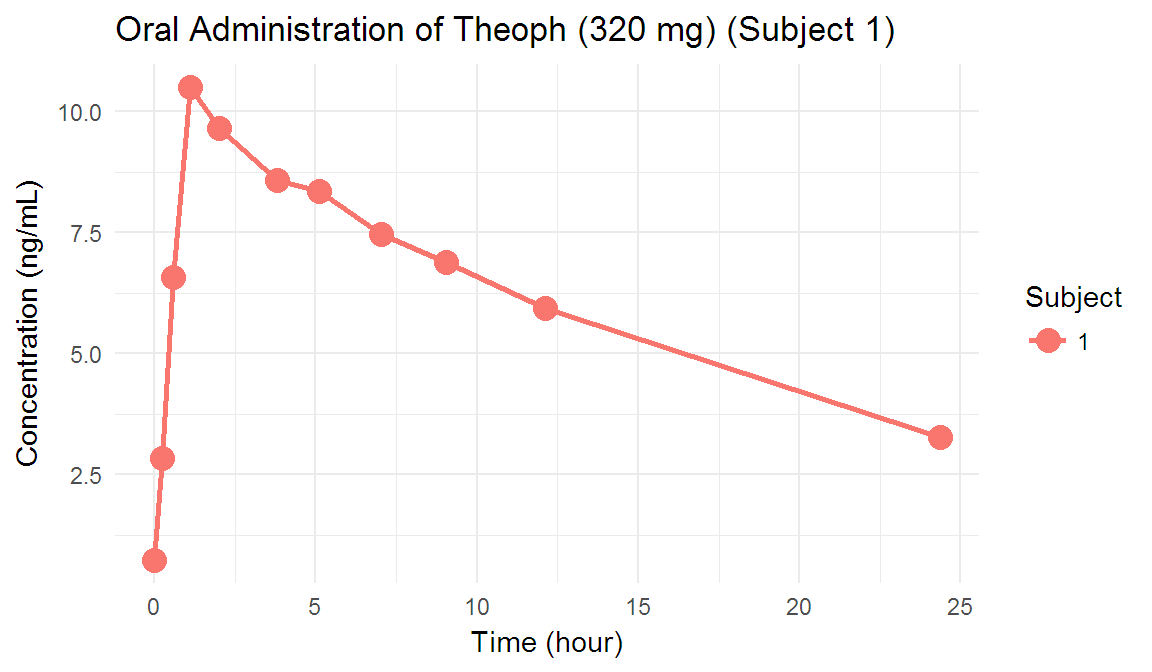
\includegraphics{handout_files/figure-latex/ggtheophindi-1.pdf}
\caption{\label{fig:ggtheophindi}Individual concentration-time curves of
oral administration of Theoph (Subject 1)}
\end{figure}

\hypertarget{tblnca----}{%
\section{tblNCA(): 전체 대상자 비구획 분석}\label{tblnca----}}

가장 많이 쓰는 함수 입니다! NonCompart 패키지의 핵심적인 기능입니다.
아래의 코드를 R의 콘솔창에 넣어보세요. 테오필린 경구 투여시의 비구획
분석입니다.

\begin{Shaded}
\begin{Highlighting}[]
\NormalTok{Theoph_tblNCA <-}\StringTok{ }\KeywordTok{tblNCA}\NormalTok{(Theoph, }\DataTypeTok{key=}\StringTok{"Subject"}\NormalTok{, }\DataTypeTok{dose=}\DecValTok{320}\NormalTok{, }\DataTypeTok{concUnit=}\StringTok{"mg/L"}\NormalTok{)}
\end{Highlighting}
\end{Shaded}

결과는 matrix 형태인데 너무 길기 때문에 핵심적인 일부 파라메터
(C\textsubscript{max}, T\textsubscript{max}, AUC\textsubscript{last})만
표시할 수도 있습니다.

\begin{Shaded}
\begin{Highlighting}[]
\NormalTok{Theoph_tblNCA_selected <-}\StringTok{ }\NormalTok{Theoph_tblNCA[ , }\KeywordTok{c}\NormalTok{(}\StringTok{'Subject'}\NormalTok{, }\StringTok{'CMAX'}\NormalTok{, }\StringTok{'TMAX'}\NormalTok{, }\StringTok{'AUCLST'}\NormalTok{)]}
\NormalTok{Theoph_tblNCA_selected}
\end{Highlighting}
\end{Shaded}

\begin{verbatim}
##       Subject CMAX    TMAX   AUCLST     
##  [1,] "1"     "10.5"  "1.12" "148.92305"
##  [2,] "2"     "8.33"  "1.92" "91.5268"  
##  [3,] "3"     "8.2"   "1.02" "99.2865"  
##  [4,] "4"     "8.6"   "1.07" "106.7963" 
##  [5,] "5"     "11.4"  "1"    "121.2944" 
##  [6,] "6"     "6.44"  "1.15" "73.77555" 
##  [7,] "7"     "7.09"  "3.48" "90.7534"  
##  [8,] "8"     "7.56"  "2.02" "88.55995" 
##  [9,] "9"     "9.03"  "0.63" "86.32615" 
## [10,] "10"    "10.21" "3.55" "138.3681" 
## [11,] "11"    "8"     "0.98" "80.0936"  
## [12,] "12"    "9.75"  "3.52" "119.9775"
\end{verbatim}

인도메타신 정맥 투여시의 비구획 분석입니다. 함수인자 \texttt{adm}을
infusion으로 바꾼 것을 볼 수 있고 \texttt{dur}가 추가된 것을 볼 수
있습니다.

\begin{Shaded}
\begin{Highlighting}[]
\NormalTok{Indometh_tblNCA <-}\StringTok{ }\KeywordTok{tblNCA}\NormalTok{(Indometh, }\DataTypeTok{key=}\StringTok{"Subject"}\NormalTok{, }\DataTypeTok{colTime=}\StringTok{"time"}\NormalTok{, }\DataTypeTok{colConc=}\StringTok{"conc"}\NormalTok{, }\DataTypeTok{dose=}\DecValTok{25}\NormalTok{, }
       \DataTypeTok{adm=}\StringTok{"Infusion"}\NormalTok{, }\DataTypeTok{dur=}\FloatTok{0.5}\NormalTok{, }\DataTypeTok{concUnit=}\StringTok{"mg/L"}\NormalTok{)}
\end{Highlighting}
\end{Shaded}

역시 핵심적인 일부 파라메터 (C\textsubscript{max}, T\textsubscript{max},
AUC\textsubscript{last})만 표시할 수도 있습니다.

\begin{Shaded}
\begin{Highlighting}[]
\NormalTok{Indometh_tblNCA_selected <-}\StringTok{ }\NormalTok{Indometh_tblNCA[ , }\KeywordTok{c}\NormalTok{(}\StringTok{'Subject'}\NormalTok{, }\StringTok{'CMAX'}\NormalTok{, }\StringTok{'TMAX'}\NormalTok{, }\StringTok{'AUCLST'}\NormalTok{)]}
\NormalTok{Indometh_tblNCA_selected}
\end{Highlighting}
\end{Shaded}

\begin{verbatim}
##      Subject CMAX   TMAX   AUCLST   
## [1,] "1"     "1.5"  "0.25" "1.74125"
## [2,] "2"     "2.03" "0.25" "2.9325" 
## [3,] "3"     "2.72" "0.25" "2.93375"
## [4,] "4"     "1.85" "0.25" "2.4775" 
## [5,] "5"     "2.05" "0.25" "1.95375"
## [6,] "6"     "2.31" "0.25" "2.8725"
\end{verbatim}

\hypertarget{-descriptive-statistics}{%
\section{기술통계 (Descriptive
statistics)}\label{-descriptive-statistics}}

R에서는 필요에 따라서 자신만의 함수를 만들 수도 있습니다. 아래 두줄을
실행하면 \texttt{desc\_tblNCA()} 함수를 사용하여 기술통계량을 쉽게 구할
수 있습니다. (Table \ref{tab:theodesc} and \ref{tab:indodesc})

\begin{Shaded}
\begin{Highlighting}[]
\NormalTok{desc_tblNCA <-}\StringTok{ }\ControlFlowTok{function}\NormalTok{(tblNCA)\{}\KeywordTok{as.data.frame}\NormalTok{(tblNCA) }\OperatorTok\StringTok{ }
\StringTok{    }\KeywordTok{mutate_all}\NormalTok{(}\ControlFlowTok{function}\NormalTok{(x) }\KeywordTok{as.numeric}\NormalTok{(}\KeywordTok{as.character}\NormalTok{(x))) }\OperatorTok\StringTok{ }\NormalTok{broom}\OperatorTok{::}\KeywordTok{tidy}\NormalTok{()\}}
\end{Highlighting}
\end{Shaded}

\begin{Shaded}
\begin{Highlighting}[]
\KeywordTok{desc_tblNCA}\NormalTok{(Theoph_tblNCA_selected)}
\KeywordTok{desc_tblNCA}\NormalTok{(Indometh_tblNCA_selected)}
\end{Highlighting}
\end{Shaded}

\begin{table}

\caption{\label{tab:theodesc}Descriptive statistics of selected PK parameters of Theoph oral administration}
\centering
\begin{tabular}[t]{lrrrrrrrrrrrr}
\toprule
column & n & mean & sd & median & trimmed & mad & min & max & range & skew & kurtosis & se\\
\midrule
Subject & 12 & 6.500000 & 3.605551 & 6.50000 & 6.5000 & 4.447800 & 1.00000 & 12.000 & 11.0000 & 0.0000000 & -1.501603 & 1.0408330\\
CMAX & 12 & 8.759167 & 1.472959 & 8.46500 & 8.7270 & 1.623447 & 6.44000 & 11.400 & 4.9600 & 0.2137012 & -1.186397 & 0.4252066\\
TMAX & 12 & 1.788333 & 1.112408 & 1.13500 & 1.7280 & 0.489258 & 0.63000 & 3.550 & 2.9200 & 0.6998568 & -1.345075 & 0.3211245\\
AUCLST & 12 & 103.806775 & 23.645216 & 95.40665 & 102.2983 & 19.794711 & 73.77555 & 148.923 & 75.1475 & 0.5625746 & -1.117566 & 6.8257858\\
\bottomrule
\end{tabular}
\end{table}

\begin{table}

\caption{\label{tab:indodesc}Descriptive statistics of selected PK parameters of Indometh IV infusion}
\centering
\begin{tabular}[t]{lrrrrrrrrrrrr}
\toprule
column & n & mean & sd & median & trimmed & mad & min & max & range & skew & kurtosis & se\\
\midrule
Subject & 6 & 3.500000 & 1.8708287 & 3.500 & 3.500000 & 2.2239000 & 1.00000 & 6.00000 & 5.0000 & 0.0000000 & -1.797619 & 0.7637626\\
CMAX & 6 & 2.076667 & 0.4135537 & 2.040 & 2.076667 & 0.3409980 & 1.50000 & 2.72000 & 1.2200 & 0.1777485 & -1.361889 & 0.1688326\\
TMAX & 6 & 0.250000 & 0.0000000 & 0.250 & 0.250000 & 0.0000000 & 0.25000 & 0.25000 & 0.0000 & NaN & NaN & 0.0000000\\
AUCLST & 6 & 2.485208 & 0.5267325 & 2.675 & 2.485208 & 0.3826961 & 1.74125 & 2.93375 & 1.1925 & -0.3695625 & -1.940994 & 0.2150376\\
\bottomrule
\end{tabular}
\end{table}

\hypertarget{-ncar}{%
\chapter{패키지: ncar}\label{-ncar}}

보고서를 만드는 패키지입니다. 현재 설정된 working directory에 결과
파일이 생성됩니다.

\hypertarget{txtnca}{%
\section{txtNCA()}\label{txtnca}}

txtNCA()를 통해서 다음 결과를 얻을 수 있습니다.

\begin{Shaded}
\begin{Highlighting}[]
\KeywordTok{txtNCA}\NormalTok{(Theoph[Theoph}\OperatorTok{$}\NormalTok{Subject}\OperatorTok{==}\StringTok{"1"}\NormalTok{,}\StringTok{"Time"}\NormalTok{],}
\NormalTok{       Theoph[Theoph}\OperatorTok{$}\NormalTok{Subject}\OperatorTok{==}\StringTok{"1"}\NormalTok{,}\StringTok{"conc"}\NormalTok{], }
       \DataTypeTok{dose=}\DecValTok{320}\NormalTok{, }\DataTypeTok{doseUnit=}\StringTok{"mg"}\NormalTok{, }\DataTypeTok{concUnit=}\StringTok{"mg/L"}\NormalTok{, }\DataTypeTok{timeUnit=}\StringTok{"h"}\NormalTok{)}
\end{Highlighting}
\end{Shaded}

\begin{verbatim}
##  [1] "                        NONCOMPARTMENTAL ANALYSIS REPORT"                           
##  [2] "                       Package version 0.3.7 (2017-08-16 KST)"                      
##  [3] "                          R version 3.4.2 (2017-09-28)"                             
##  [4] ""                                                                                   
##  [5] "Date and Time: 2017-11-14 13:56:23 Asia/Seoul"                                      
##  [6] ""                                                                                   
##  [7] "Calculation Setting"                                                                
##  [8] "-------------------"                                                                
##  [9] "Drug Administration: Extravascular"                                                 
## [10] "Observation count excluding trailing zero: 11"                                      
## [11] "Dose at time 0: 320 mg"                                                             
## [12] "AUC Calculation Method: Linear-up Linear-down"                                      
## [13] "Weighting for lambda z: Uniform (Ordinary Least Square, OLS)"                       
## [14] "Lambda z selection criterion: Heighest adjusted R-squared value with precision=1e-4"
## [15] ""                                                                                   
## [16] ""                                                                                   
## [17] "Fitting, AUC, AUMC Result"                                                          
## [18] "-------------------------"                                                          
## [19] "      Time         Conc.      Pred.   Residual       AUC       AUMC"                
## [20] "---------------------------------------------------------------------"              
## [21] "     0.0000       0.7400                           0.0000     0.0000"               
## [22] "     0.2500       2.8400                           0.4475     0.0888"               
## [23] "     0.5700       6.5700                           1.9531     0.8015"               
## [24] "     1.1200      10.5000                           6.6474     5.0654"               
## [25] "     2.0200       9.6600                          15.7194    19.1383"               
## [26] "     3.8200       8.5800                          32.1354    66.1982"               
## [27] "     5.1000       8.3600                          42.9769   114.4617"               
## [28] "     7.0300       7.4700                          58.2529   206.2815"               
## [29] "     9.0500 *     6.8900     6.8912 -1.228e-03    72.7565   322.2988"               
## [30] "    12.1200 *     5.9400     5.9387 +1.324e-03    92.4505   528.5219"               
## [31] "    24.3700 *     3.2800     3.2801 -1.465e-04   148.9231  1459.0711"               
## [32] ""                                                                                   
## [33] "*: Used for the calculation of Lambda z."                                           
## [34] ""                                                                                   
## [35] ""                                                                                   
## [36] "Calculated Values"                                                                  
## [37] "-----------------"                                                                  
## [38] "CMAX       Max Conc                                       10.5000 mg/L"             
## [39] "CMAXD      Max Conc Norm by Dose                           0.0328 mg/L/mg"          
## [40] "TMAX       Time of CMAX                                    1.1200 h"                
## [41] "TLAG       Time Until First Nonzero Conc                   0.0000 h"                
## [42] "CLST       Last Nonzero Conc                               3.2800 mg/L"             
## [43] "CLSTP      Last Nonzero Conc Pred                          3.2801 mg/L"             
## [44] "TLST       Time of Last Nonzero Conc                      24.3700 h"                
## [45] "LAMZHL     Half-Life Lambda z                             14.3044 h"                
## [46] "LAMZ       Lambda z                                        0.0485 /h"               
## [47] "LAMZLL     Lambda z Lower Limit                            9.0500 h"                
## [48] "LAMZUL     Lambda z Upper Limit                           24.3700 h"                
## [49] "LAMZNPT    Number of Points for Lambda z                   3"                       
## [50] "CORRXY     Correlation Between TimeX and Log ConcY        -1.0000 "                 
## [51] "R2         R Squared                                       1.0000 "                 
## [52] "R2ADJ      R Squared Adjusted                              1.0000 "                 
## [53] "AUCLST     AUC to Last Nonzero Conc                      148.9231 h*mg/L"           
## [54] "AUCALL     AUC All                                       148.9231 h*mg/L"           
## [55] "AUCIFO     AUC Infinity Obs                              216.6119 h*mg/L"           
## [56] "AUCIFOD    AUC Infinity Obs Norm by Dose                   0.6769 h*mg/L/mg"        
## [57] "AUCIFP     AUC Infinity Pred                             216.6150 h*mg/L"           
## [58] "AUCIFPD    AUC Infinity Pred Norm by Dose                  0.6769 h*mg/L/mg"        
## [59] "AUCPEO     AUC %Extrapolation Obs                         31.2489 %"                
## [60] "AUCPEP     AUC %Extrapolation Pred                        31.2499 %"                
## [61] "AUMCLST    AUMC to Last Nonzero Conc                    1459.0711 h2*mg/L"          
## [62] "AUMCIFO    AUMC Infinity Obs                            4505.5348 h2*mg/L"          
## [63] "AUMCIFP    AUMC Infinity Pred                           4505.6709 h2*mg/L"          
## [64] "AUMCPEO    AUMC %Extrapolation Obs                        67.6160 %"                
## [65] "AUMCPEP    AUMC % Extrapolation Pred                      67.6170 %"                
## [66] "VZFO       Vz Obs by F                                    30.4867 L"                
## [67] "VZFP       Vz Pred by F                                   30.4863 L"                
## [68] "CLFO       Total CL Obs by F                               1.4773 L/h"              
## [69] "CLFP       Total CL Pred by F                              1.4773 L/h"              
## [70] "MRTEVLST   MRT Extravasc to Last Nonzero Conc              9.7975 h"                
## [71] "MRTEVIFO   MRT Extravasc Infinity Obs                     20.8000 h"                
## [72] "MRTEVIFP   MRT Extravasc Infinity Pred                    20.8004 h"
\end{verbatim}

파일로 저장하려면 다음을 입력합니다.

\begin{Shaded}
\begin{Highlighting}[]
\KeywordTok{writeLines}\NormalTok{(}\KeywordTok{txtNCA}\NormalTok{(Theoph[Theoph}\OperatorTok{$}\NormalTok{Subject}\OperatorTok{==}\StringTok{"1"}\NormalTok{,}\StringTok{"Time"}\NormalTok{],}
\NormalTok{                  Theoph[Theoph}\OperatorTok{$}\NormalTok{Subject}\OperatorTok{==}\StringTok{"1"}\NormalTok{,}\StringTok{"conc"}\NormalTok{], }
                  \DataTypeTok{dose=}\DecValTok{320}\NormalTok{, }\DataTypeTok{doseUnit=}\StringTok{"mg"}\NormalTok{, }\DataTypeTok{concUnit=}\StringTok{"mg/L"}\NormalTok{,}
                  \DataTypeTok{timeUnit=}\StringTok{"h"}\NormalTok{), }
           \StringTok{'Output-ncar/txtNCA-Theoph.txt'}\NormalTok{)}
\end{Highlighting}
\end{Shaded}

\hypertarget{pdfnca}{%
\section{pdfNCA()}\label{pdfnca}}

pdfNCA()로 pdf로 결과를 볼 수 있습니다.

\begin{Shaded}
\begin{Highlighting}[]
\KeywordTok{pdfNCA}\NormalTok{(}\DataTypeTok{fileName=}\StringTok{"Output-ncar/pdfNCA-Theoph.pdf"}\NormalTok{, Theoph, }\DataTypeTok{colSubj=}\StringTok{"Subject"}\NormalTok{, }\DataTypeTok{colTime=}\StringTok{"Time"}\NormalTok{, }
       \DataTypeTok{colConc=}\StringTok{"conc"}\NormalTok{, }\DataTypeTok{dose=}\DecValTok{320}\NormalTok{, }\DataTypeTok{doseUnit=}\StringTok{"mg"}\NormalTok{, }\DataTypeTok{timeUnit=}\StringTok{"h"}\NormalTok{, }\DataTypeTok{concUnit=}\StringTok{"mg/L"}\NormalTok{)}
\end{Highlighting}
\end{Shaded}

\begin{verbatim}
## pdf 
##   2
\end{verbatim}

\hypertarget{rtfnca}{%
\section{rtfNCA()}\label{rtfnca}}

마이크로소프트 워드에서 편집가능한 rtf파일을 만듭니다.

\begin{Shaded}
\begin{Highlighting}[]
\KeywordTok{rtfNCA}\NormalTok{(}\DataTypeTok{fileName=}\StringTok{"rtfNCA-Theoph.rtf"}\NormalTok{, Theoph, }\DataTypeTok{colSubj=}\StringTok{"Subject"}\NormalTok{, }\DataTypeTok{colTime=}\StringTok{"Time"}\NormalTok{, }
       \DataTypeTok{colConc=}\StringTok{"conc"}\NormalTok{, }\DataTypeTok{dose=}\DecValTok{320}\NormalTok{, }\DataTypeTok{doseUnit=}\StringTok{"mg"}\NormalTok{, }\DataTypeTok{timeUnit=}\StringTok{"h"}\NormalTok{, }\DataTypeTok{concUnit=}\StringTok{"mg/L"}\NormalTok{)}
\end{Highlighting}
\end{Shaded}

\hypertarget{-pkr}{%
\chapter{패키지: pkr}\label{-pkr}}

\hypertarget{plotpk}{%
\section{plotPK()}\label{plotpk}}

여러가지 기본적인 그림을 그려봅니다. Output 폴더 아래에 여러 파일이
생성됩니다.

\begin{Shaded}
\begin{Highlighting}[]
\NormalTok{pkr}\OperatorTok{::}\KeywordTok{plotPK}\NormalTok{(Theoph, }\StringTok{"Subject"}\NormalTok{, }\StringTok{"Time"}\NormalTok{, }\StringTok{"conc"}\NormalTok{, }
            \DataTypeTok{unitTime =} \StringTok{"hr"}\NormalTok{, }\DataTypeTok{unitConc =} \StringTok{"mg/L"}\NormalTok{, }\DataTypeTok{dose =} \DecValTok{320}\NormalTok{)}
\end{Highlighting}
\end{Shaded}

\begin{verbatim}
## pdf 
##   2
\end{verbatim}

\hypertarget{etc}{%
\chapter{기타 사항}\label{etc}}

\hypertarget{shiny-}{%
\section{shiny 앱}\label{shiny-}}

웹브라우저를 통해 간단히 비구획분석을 할 수 있는 앱을 개발하였습니다.

\begin{itemize}
\tightlist
\item
  Han, S. (2017) pkrshiny: Noncompartmental Analysis using pkr R package
  Shiny application. URL: \url{https://asan.shinyapps.io/pkrshiny}
\end{itemize}

그 외 약동학과 관련된 몇가지 shiny 앱도 참고하세요.

\begin{itemize}
\tightlist
\item
  Han, S. (2017) Pharmacokinetic Simulation of one-compartment Models.
  URL: \url{https://asan.shinyapps.io/pk1c/}
\item
  Han, S. (2017) caff: Monte Carlo Simulation of Caffeine Shiny
  application. URL: \url{https://asan.shinyapps.io/caff}
\item
  Han, S. (2016) vtdm: Vancomycin TDM Shiny application. URL:
  \url{https://asan.shinyapps.io/vtdm}
\end{itemize}

\section{지원}

패키지와 관련한 모든 의문은
\href{mailto:shan@acp.kr}{\nolinkurl{shan@acp.kr}} / 02-3010-4614 으로
연락 주시면 빠르게 도움 드리겠습니다. 혹은 StackOverflow\footnote{\url{https://stackoverflow.com}}에
영어로 질문 올려주시고 링크를 보내주시면 더 좋습니다. 아직 미완성이지만
Gitbook (일종의 웹북)\footnote{\url{https://asancpt.github.io/book-ncar}}을
통해 전자출판도 진행 중이므로 시간 나실때 틈틈이 확인해 주시면
감사하겠습니다. (Figure \ref{fig:gitbook})

서울아산병원 임상약리학과 전공의 한성필

\begin{figure}
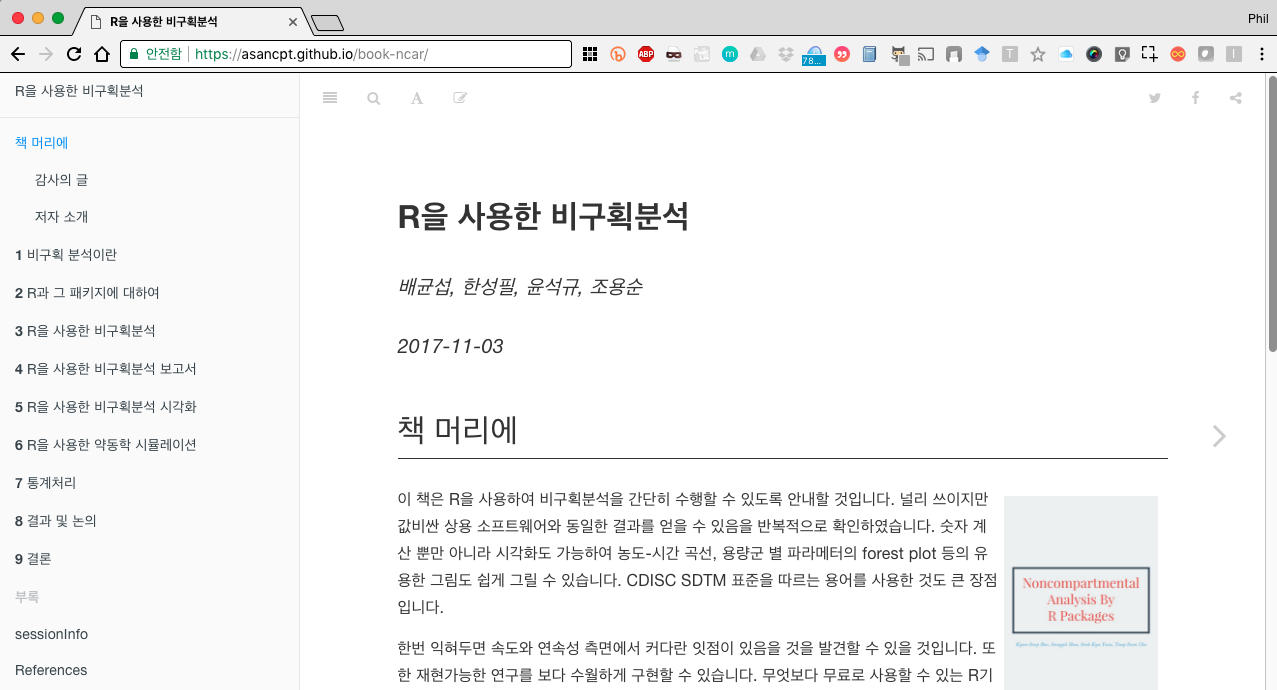
\includegraphics[width=400px]{assets/gitbook} \caption{Gitbook: Noncompartmental analysis by R (work in progress)}\label{fig:gitbook}
\end{figure}

\section{고지}

본 출판물은 2016, 2017년도 정부(미래창조과학부)의 재원으로 한국연구재단
첨단 사이언스·교육 허브 개발 사업의 지원을 받아 수행된 결과입니다
(NRF-2016-936606).

\hypertarget{references}{%
\chapter{참고문헌}\label{references}}

\hypertarget{refs}{}
\leavevmode\hypertarget{ref-R-ncar}{}%
Bae, Kyun-Seop. 2017a. \emph{Ncar: Noncompartmental Analysis for
Pharmacokinetic Report}. \url{https://CRAN.R-project.org/package=ncar}.

\leavevmode\hypertarget{ref-R-NonCompart}{}%
---------. 2017b. \emph{NonCompart: Noncompartmental Analysis for
Pharmacokinetic Data}.
\url{https://CRAN.R-project.org/package=NonCompart}.

\leavevmode\hypertarget{ref-R-pkr}{}%
Bae, Kyun-Seop, and Jee Eun Lee. 2017. \emph{Pkr: Pharmacokinetics in
R}. \url{https://CRAN.R-project.org/package=pkr}.

\leavevmode\hypertarget{ref-R-base}{}%
R Core Team. 2017. \emph{R: A Language and Environment for Statistical
Computing}. Vienna, Austria: R Foundation for Statistical Computing.
\url{https://www.R-project.org/}.


\end{document}
